\chapter{Определение длины световой волны по картине дифракции на круглом отверстии}

\section{Цель работы}

Определение длины световой волны по картине дифракции на малом круглом отверстии

\section{Ход работы}

Координата объектива $X_\infty = 83.4$.

\begin{table}[H]
	\centering
	\caption{Замеры}
	\begin{tabular}{|c|c|c|c|}
		\hline
		$m$ & $X_{o1}$ & $X_{o2}$ & $X_{o3}$ \\ \hline
		2 & 64 & 64.7 & 64.5 \\ \hline
		3 & 70.5 & 70.1 & 70.7 \\ \hline
		4 & 73.6 & 73.4 & 73.5 \\ \hline
		5 & 75.7 & 75.6 & 75.7 \\ \hline
		6 & 77 & 77 & 77.1 \\ \hline
	\end{tabular}
\end{table}

\[
d=l-b=x_\infty-x
\]
\begin{table}[H]
	\centering
	\caption{Расчёты}
	\begin{tabular}{|c|c|c|c|}
		\hline
		$m$ & $d_1$ & $d_2$ & $d_3$ \\ \hline
		2 & 19.4 & 18.7 & 18.9 \\ \hline
		3 & 12.9 & 13.3 & 12.7 \\ \hline
		4 & 9.8 & 10 & 9.9 \\ \hline
		5 & 7.7 & 7.8 & 7.7 \\ \hline
		6 & 6.4 & 6.4 & 6.3 \\ \hline
	\end{tabular}
\end{table}

\begin{table}[H]
	\centering
	\caption{Зависимость}
	\begin{tabular}{|c|c|c|c|c|c|}
		\hline
		$\frac{1}{m}$ & $\frac{1}{6}$ & $\frac{1}{5}$ & $\frac{1}{4}$ & $\frac{1}{3}$ & $\frac{1}{2}$ \\ \hline
		$d$ & 6.37 & 7.73 & 9.9 & 12.97 & 19 \\ \hline
	\end{tabular}
\end{table}

\begin{landscape}
	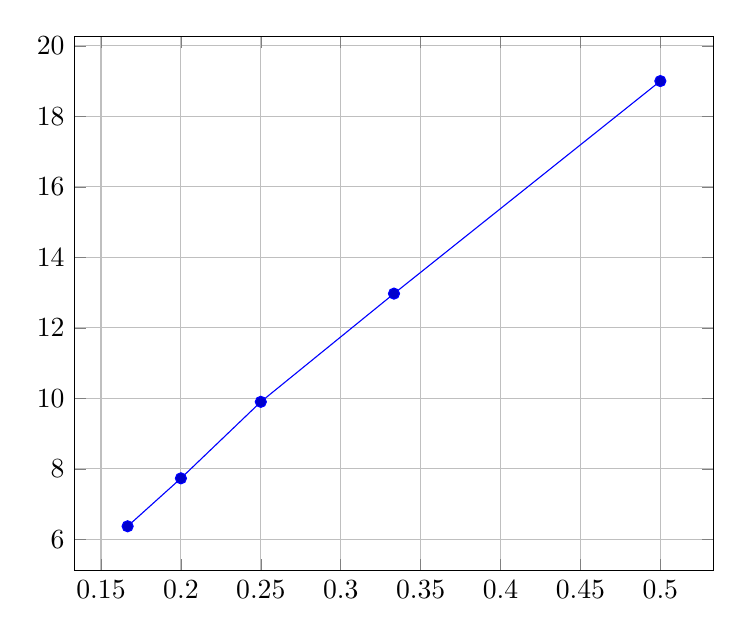
\begin{tikzpicture}
	\begin{axis}[grid=both,
	width=0.8\linewidth]
	\addplot coordinates {
		(1/6, 6.37)
		(1/5, 7.73)
		(1/4, 9.9)
		(1/3, 12.97)
		(1/2, 19)		
	};
	\end{axis}
	
	\end{tikzpicture}
\end{landscape}

Уравнение аппроксимирующей прямой:

\[
y=37.7309 \cdot x + 0.252045
\] 

Длина световой волны:

\[
\lambda = \frac{r^2}{k} = \frac{(0.5*10^{-1})^2}{37.7309} = 662 \text{нм}
\]

Погрешность наклона $\Delta K$:

\[
\Delta K = \sqrt{(k-k_1)^2+(k-k_2)^2+(k-k_3)^2+(k-k_4)^2} = 0.0182
\]

\[
\Delta \lambda = \sqrt{\frac{0.0005^2}{37.739^2}+\frac{2*0.0005}{37.739}} \approx 53.3 \text{ нм}
\]


Длина волны с учётом погрешности:

\[
\lambda = 662 \pm 53.3 \text{ нм}
\]